\chapter{Results}
\label{ch:intro}

\section{Activities and working patterns}
For the first part of this section we present a characterization of working sessions at different levels, extracting the information from ABB's dataset. As this data corresponds to full-time developers, it is safe to assume that they follow certain working patterns and have common activities, so we expect to see an homogeneous behavior among the developers.

In contrast, UDC's dataset contains more variety and different profiles of programmers, which could be troublesome when trying to find a common set of activities.

\subsection{Characterizing working sessions}
We defined a working session as a lapse of recorded activity surrounded by interruptions of large duration (8 hours), to model a day of work. However, in many cases the extracted sessions contained an interruption of moderate length in the middle, so we set the threshold to 4 hours to split this kind of sessions. At the end, we had 1,585 sessions with an average duration of 4.7 hours ($s=3.58$).

From the transformation phase, every session is composed of time series and other attributes. There is a time series to represent the interruptions, where the amplitude is the duration of every interruption, and 11 more series whose amplitude is the amount of events of every type per minute. Every data point of the time series is equal to a minute of activity in the data, meaning that all the time series have the same length. In average this length is of $121.61$ minutes ($s=147.81$). This is also refereed as productive time, or the total time that the programmer spent working on the IDE without being interrupted.

A lot of the time of a working session is wasted in interruptions, or time segments of at least 3 minutes without recorded activity. In average every session has 18 interruptions (sd=21.17) with an average duration of 10.78 minutes. As for the total time consumed in interruptions, the average is of 190 minutes (sd=137.19), which is more than half the average duration of a session.

\subsection{Using focus data}
Complementary to the dataset, we had access to the focus data of a smaller group of programmers from ABB. This dataset contains the focus level (a value between 0 and 1) per minute that Codealike uses in its tool as an inference of the concentration of the user. The focus is calculated according to two functions: one to increase the value when the programmer makes use of the IDE, and a second one as a decay function, that is applied when the programmer is inactive. Therefore, when the user is active the value decreases and the contrary when he is not using the IDE.

This can be used as a summarization of the activity the user and to get very general information. For example, the Figure \ref{fig:prod_hours} shows the total focus per hour from all the programmers. We can see that the 14 hours seems to be the more productive time, for is the hour with the higher value of focus or the time with more usage of the IDE. There is a decrease at the 16 hrs., and increases a again to later abruptly drop at 21 hrs. The activity is lower between the 21 and 8 hours.

\begin{figure}[!ht]
	\centering
	\begin{tabular}{c}
		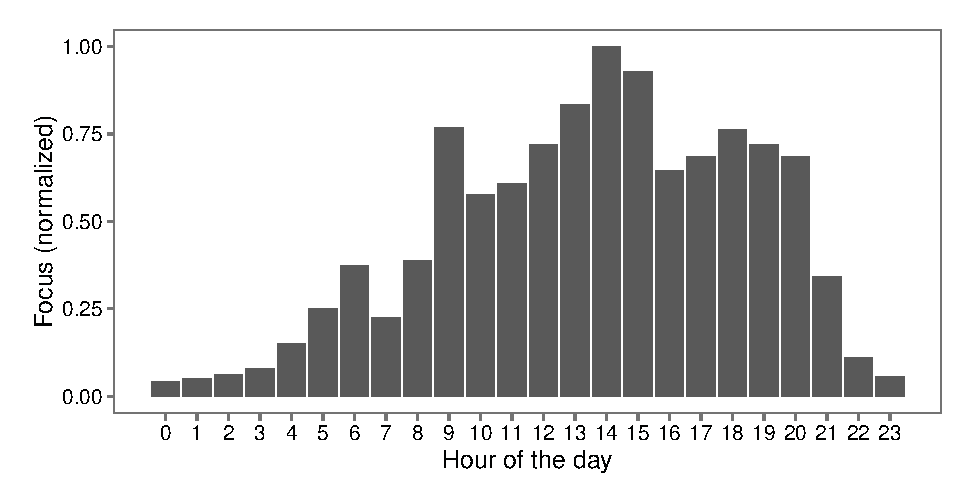
\includegraphics[width=1\linewidth,clip=, angle=0]{Figures/productive_hours_focus} 
	\end{tabular}
	\caption{Histogram of productivity per hour according to the focus data.}
	\label{fig:prod_hours}
\end{figure}

With this information we can also see the evolution of productivity throughout the days of the week. The Figure \ref{fig:prod_days} shows the sum of focus level (normalized) for every day of the week. There is not a great difference aside from the weekend, but there is a slight decrease the days Monday and Friday, and the most productive days are Tuesday and Thursday.

\begin{figure}[!ht]
	\centering
	\begin{tabular}{c}
		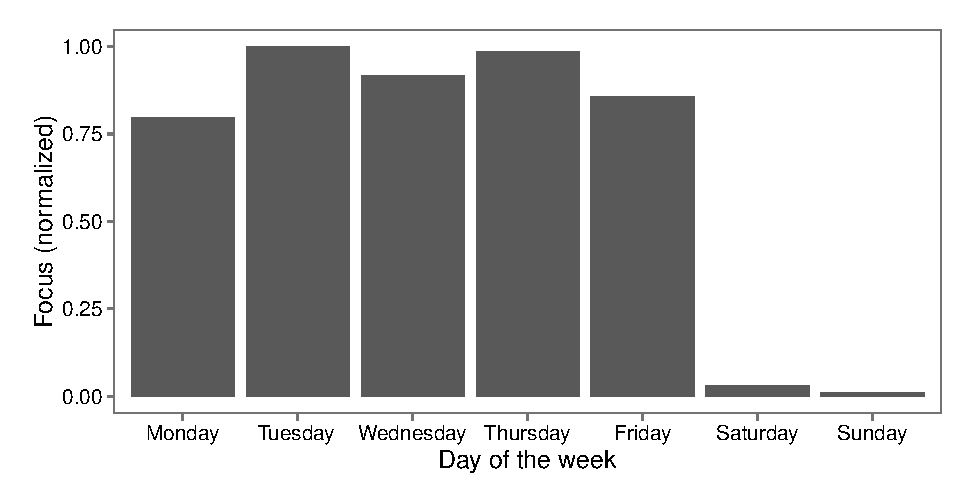
\includegraphics[width=1\linewidth,clip=, angle=0]{Figures/productive_days_focus} 
	\end{tabular}
	\caption{Histogram of productivity per day according to the focus data.}
	\label{fig:prod_days}
\end{figure}

%\subsection{Decomposed working sessions}
%To explore the working patterns at a finer level, we decomposed the sessions to small chunks of 3 to 5 minutes of activity without interruptions. This resulted in 31,973 different observations, each with their respective time series and proportion of events by type. 

%\subsection{Characterizing developers}
%We have information from 69 programmers, each offering an average of 22 working sessions. We do not have more information about them, like roles and working hours

\subsection{Identifying types of activities}
In order to identify the types of activities the programmers perform, we split every working session into smaller activity time frames of 3 to 5 minutes of length. For each of this new chunks of the sessions we recreated the time series and calculated the proportion of events per type, which is the count of events of type $t$ divided by the total count of events in that chunk. After this, we obtained a total of 31,727 chunks.

The nature (or the type) of a chunk is defined by the amount of events of certain type in comparison with others. For example, for the activity of programming we expect a high proportion of events of edition, and probably also navigation around text and classes. The challenge is to know what threshold set to differentiate between two types of activities that might use the same kind of events, i.e. reading and programming could both use text navigation events. Also, if we try to define a set of activities according to experience and related work, we might be ignoring certain characteristic activities of this group of programmers or forcing one to exist. For this reasons we decided to implement clustering algorithms with the chunks, taking the proportion of events as the attributes. So, every observation contained 11 different attributes whose values are between 0 and 1.

As we didn't know how many types of activities there were, we discarded the algorithms that require the number of clusters as parameter, like K-means and K-medians. From the rest of algorithms, we chose Mean shift because: (1) in contrast with Affinity propagation (our other option) the time complexity is lower, and (2) the Mean shift technique performs one last step to unify very similar clusters. The importance of the second point will be discussed later.

An issue with Mean shift is that the size of the observations has a big impact in the results: a small population can offer more variety of clusters, and a big population could be clustered around one or two centers. Mean shifts creates the clusters by estimating a density function over a region of size given by the bandwidth, a parameter of the algorithm. So, the bandwidth also has an effect on the results.

It is difficult to know which are the appropriate parameters and sample size because, for we do not know what are the results. To tackle this, we took the following approach:
\begin{enumerate}
	\item From the observations, select a random sample size $n$.
	\item Execute the Mean shift technique with the random sample.
	\item Store the resulting clusters.
	\item Repeat $k$ times steps 1 to 3.
	\item Filter the clusters to eliminate very close centers according to the Euclidean distance and a threshold $d$. 
	\item Discard clusters that only appeared in one execution.
\end{enumerate}

The fifth step is done by measuring the distance of a cluster with the rest and selecting the group of clusters with a distance lesser or equal to $d$. Then, we calculated the median of the attributes of all the clusters in that group and substituted the group with the new cluster created from the medians. 

With this approach we were able to observe very common clusters corresponding to frequent activities like programming and debugging, and also activities that only occur on special occasions or that are not very common within a working session.


With $n=300$ and $k=150$, the Table \ref{tbl:activities} shows the resulting clusters. We selected the corresponding activity by inspecting the closeness of the center to the attributes: the higher the value, the most events of that type. For example the Debugging activity has a value of 0.90 (from a range between 0 to 1) for the debug type; the rest of the activities have a value $<0.20$ for that type of event. Next, we describe each of the activities discovered via clustering:

\begin{itemize}
	\item \emph{Debugging}. The most common activity has a big value for the debug type (0.90). It is composed of events meant to execute and control debugging sessions.
	\item \emph{Programming}. It has the greatest values for the edit and text-nav types (0.62 and 0.24, respectively). It contains text edition and text navigation events and it's the second most common activity.
	\item \emph{Navigation}. This activity has a high value for the high-nav type (0.85). It is often related to comprehension tasks.
	\item \emph{Version-control}. It has a high value for the control type (0.89).
	\item \emph{File-management}. It has a high value for the file type (0.86).
	\item \emph{Tool-usage}. This activity represents the execution and usage of tools within the IDE with different objectives i.e. the management of databases, user interface design and architecture diagrams design. It has a high value for the tools type (0.91)
	\item \emph{Search}. It has the higher value for the search type (0.91) and to a lesser extent for edition and text-nav (0.10 and 0.11 respectively).
	\item \emph{Refactoring}. It has a high value for the refactoring type (0.90) and to a lesser extent for edition, text-nav and high-nav (0.13, 0.15 and 0.13 respectively)
	\item \emph{Testing}. It has a high value for the testing type (0.95) and to a lesser extent control and file types (0.35 and 0.19 respectively).
\end{itemize}

\begin{table}
	\caption{Activities found via clustering.}
	\label{tbl:activities}
	\centering
	\begin{tabular}{c c c c}
		\hline 
		\emph{Activity} & \emph{Amount of chunks} & \emph{Users} & \emph{Times found}\\  
		\hline 
		\hline 
		Debugging & 40.62 \% & 59 & 150\\
		\hline
		Programming & 35.53 \% & 58 & 150 \\
		\hline
		Navigation & 18.67 \% & 61 & 140\\
		\hline
		Version-control & 1.85 \% & 33 & 150\\
		\hline
		File-management & 1.60 \% & 45 & 2 \\
		\hline
		Tool-usage & 0.59 \% & 28 & 149\\
		\hline
		Search & 0.49 \% & 32 & 14\\
		\hline
		Refactoring & 0.34 \% & 13 & 17\\
		\hline
		Testing & 0.30 \% & 17 & 58\\
		\hline
	\end{tabular}
\end{table}

Once we had every chunk of a session labeled with the corresponding activity, we did an analysis of the evolution of the activities throughout a working session. For that, we split every session into 10 phases and counted the activities by type on each of the phases from all the sessions. The Figure \ref{fig:activities_phases} shows a line plot with the evolution of four selected activities (Programming, Debugging, Version-control and Testing) throughout the 10 phases of the sessions.

\begin{figure}[!ht]
	\centering
	\begin{tabular}{c}
		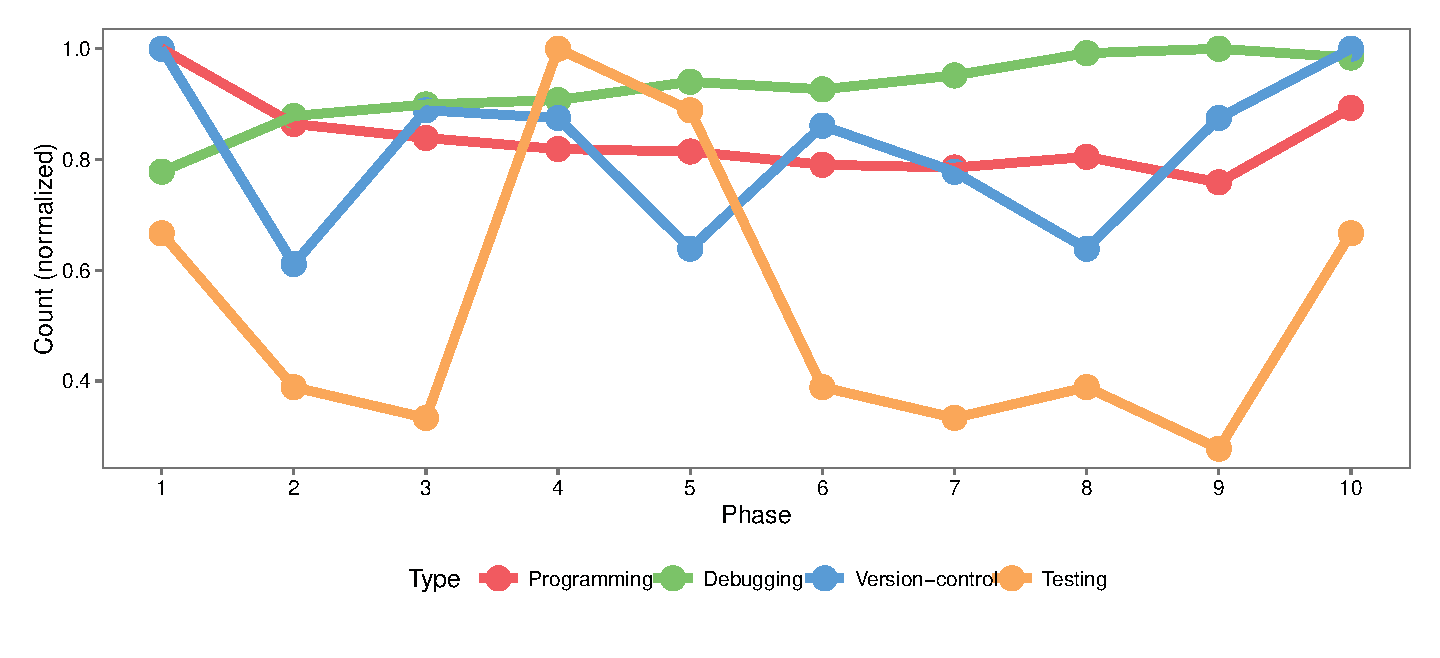
\includegraphics[width=1\linewidth,clip=, angle=0]{Figures/activities_phases} 
	\end{tabular}
	\caption{Evolution of the activities throughout the sessions.}
	\label{fig:activities_phases}
\end{figure}

We can observe that Programming starts high and gradually decreases towards the end of the session, and the contrary occurs with Debugging, whose highest point is at the 9th phase. There is a negative correlation between these two activities ($r=-0.76$), possibly meaning that as the programmer advances with the task the programming necessities are reduced but increases the need for debugging and checking the correctness of the program. In contrast, the Navigation activity (not shown in the plot) has a positive correlation with programming ($r=0.74$).

The Version-control activity seems to have an irregular behavior, being high at the beginning and ending of the session. The reason could be that at the beginning the programmer obtains the latest version of the program, while at the end he commits the final version after the working session. In the middle there are some peaks that might be different checkpoints that the programmer reaches as he has progress in the task. 

As for the Testing activities, there s an obvious peak at the middle of the session and lower activity in the rest.
